\documentclass[border=3pt]{standalone}
% Preâmbulo compartilhado pelos diagramas TikZ da aula
\usepackage[T1]{fontenc}
\usepackage[utf8]{inputenc}
\usepackage{lmodern}
\usepackage{amsmath}
\usepackage{xcolor}
\usepackage{tikz}
\usetikzlibrary{arrows.meta,angles,quotes,decorations.pathmorphing,calc,
                positioning,shapes.geometric,backgrounds,fit}

% Paleta (mesma dos SVGs originais)
\definecolor{dblue}{HTML}{2A5B8C}
\definecolor{dorange}{HTML}{B3541E}
\definecolor{dgreen}{HTML}{4A7C59}
\definecolor{dred}{HTML}{9C4B4B}
\definecolor{dcream}{HTML}{F4F1EA}
\definecolor{dshade}{HTML}{DDD7C9}

% Estilos comuns (prefixo d... para não colidir com chaves internas do pgf)
\tikzset{
  >={Stealth[length=2mm]},
  dguide/.style={gray!55, dashed, line width=0.4pt},
  daxis/.style={gray!60, line width=0.7pt, ->},
  dbody/.style={fill=black!3, draw=black!80, line width=1pt},
  dacc/.style={draw=dblue, line width=1pt},
  dlbl/.style={black!55, font=\small},
  dsub/.style={black!45, font=\footnotesize},
  dstate/.style={circle, draw=black!80, fill=dcream, line width=1pt,
                 minimum size=17mm, font=\large, inner sep=1pt},
  dobs/.style={circle, draw=black!80, fill=dshade, line width=1pt,
               minimum size=14mm, font=\large, inner sep=1pt},
  dbox/.style={rounded corners=2pt, draw=black!80, fill=dcream, line width=1pt,
               align=center, inner sep=6pt},
  dtrans/.style={->, dblue, line width=1pt},
  dmeas/.style={->, dorange, line width=1pt},
}

\begin{document}
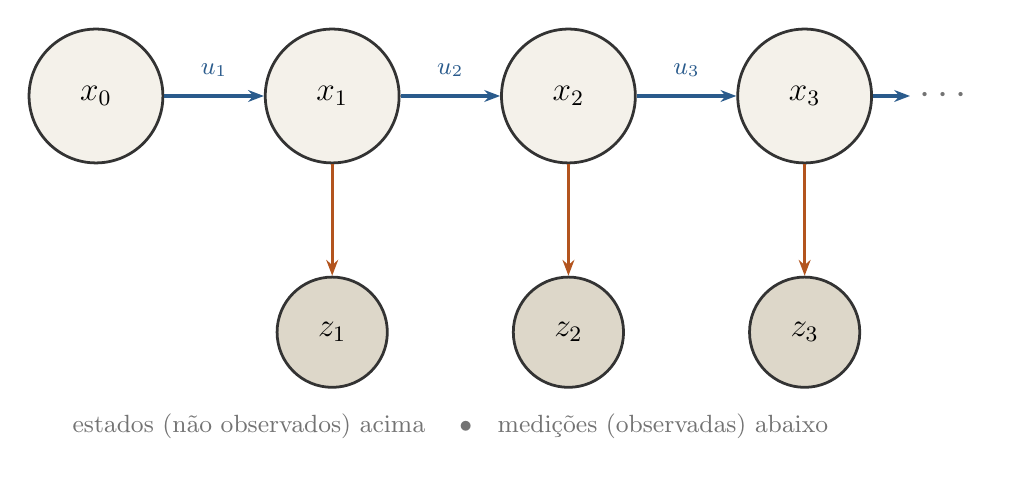
\begin{tikzpicture}[x=1cm,y=1cm]

  % estados
  \foreach \i in {0,1,2,3}
    \node[dstate] (x\i) at (3*\i,0) {$x_{\i}$};
  \node[black!55, font=\Large] (xdots) at (10.8,0) {$\cdots$};

  % transições com u
  \foreach \a/\b/\u in {x0/x1/1, x1/x2/2, x2/x3/3}
    \draw[dtrans, line width=1.1pt] (\a) -- (\b)
          node[midway, above=3pt, dblue, font=\small] {$u_{\u}$};
  \draw[dtrans, line width=1.1pt] (x3) -- (xdots);

  % medições
  \foreach \i in {1,2,3}{
    \node[dobs] (z\i) at (3*\i,-3) {$z_{\i}$};
    \draw[dmeas, line width=1.1pt] (x\i) -- (z\i);
  }

  \node[dlbl] at (4.5,-4.2)
    {estados (não observados) acima \quad$\bullet$\quad medições (observadas) abaixo};

\end{tikzpicture}
\end{document}
